\documentclass[a4paper,10pt]{article}
%\documentclass[a4paper,10pt]{scrartcl}

\usepackage[utf8]{inputenc}
\usepackage{graphicx}
\usepackage{amssymb}
\usepackage{amsmath}
\usepackage[colorlinks=true, linkcolor=black]{hyperref}
\usepackage{setspace}
\usepackage{listings}
\usepackage{color}
\usepackage{pxfonts}
\usepackage{tikz}
\usetikzlibrary{arrows,shapes,automata,backgrounds,petri}

\title{Model checking locale per aCTL}
\author{A. Rizzo, M. Bruni}
\date{18-02-2013}

\pdfinfo{
  /Title    (Model checking locale per aCTL)
  /Author   (A. Rizzo, M. Bruni)
  /Creator  (A. Rizzo, M. Bruni)
  /Producer ()
  /Subject  ()
  /Keywords ()
}

\definecolor{listinggray}{gray}{0.92}
% % % % % % % % % % % % % %
%% PRISM CODE LISTING ********************************************* 

\definecolor{prismgreen}{rgb}{0, 0.6, 0} 

\lstdefinelanguage{Checker}{ % syntax highlight via font 
        basicstyle=\color{black}\tiny\ttfamily, % small true type font (like courier) 
        keywords={bool, switch, foreach, return, if, then, else, var, case},
        keywordstyle={\bfseries\color{black}}, 
        numberstyle=\tiny\color{black}, 
        comment=[l]{//}, 
        morecomment=[s]{/*}{*/}, % single and multi-line 
        commentstyle= \color{prismgreen}\raggedleft, % dark green 
        tabsize=4, % tab treatment (going to be fixed in Prism) 
        captionpos=b, % put captions at the bottom 
        escapechar=@ % write LaTeX comments escaped by @ symbol 
} 
\newcommand*{\Comment}[1]{\hfill\makebox[3.0cm][l]{#1}}%
\renewcommand{\lstlistingname}{Code}

%% END PRISM CODE LISTING ********************************************* 

\definecolor{light-gray}{gray}{0.85}
\definecolor{lbcolor}{rgb}{0.9,0.9,0.9}

% stile per linguaggio PRISM
\lstset{ 
	backgroundcolor=\color{light-gray},
	language={Checker}, 
	numbers=left, 
	frame=shadowbox, %lines,
	rulesepcolor=\color{black}, 
	rulecolor=\color{black},
	breaklines=true, 
	breakatwhitespace=true,
	firstnumber=1, 
	firstline=1,
	lastline=25,
	xleftmargin=20pt
}



\begin{document}

%%%%%%%%%%%%%%%%%		 Frontespizio		%%%%%%%%%%%%%%%%%

\begin{titlepage}
\thispagestyle{empty}
\topmargin=1cm
\large

\begin{figure}[ht]
\centering

\includegraphics[scale=0.075]{img/Stemma.jpg}
\end{figure}

\begin{center}

UNIVERSITÀ DEGLI STUDI DI FIRENZE
\vspace{0.5cm}

Laurea Magistrale in Ingegneria Informatica
\\
\normalsize
Corso di Metodi Formali per la Verifica di Sistemi
\vspace{4cm}

\begin{huge}
Model checking locale per aCTL
\end{huge}

\vspace{0.5cm}

A. Rizzo, M. Bruni

\vspace{6cm}
\rule{6cm}{.4pt}
\\
Anno accademico 2012/2013
\end{center}
\end{titlepage}

%%%%%%%%%%%%%%%%%		End Frontespizio		%%%%%%%%%%%%%%%%%

\doublespacing

\tableofcontents % Indice

\vspace{4cm}
%Insert Creative Commons Artwork
\DeclareGraphicsExtensions{.pdf,.png,.jpg}
\begin{center}
\leavevmode
%Insert image file name below "cc-by-nc-nd.png"

\includegraphics[width=1in]{img/by-nc.png}
\end{center}
\label{fig:cc}
%insert a link to the licence and its description below
\begin{center}
\scriptsize{This document is licensed under a \href{http://creativecommons.org/licenses/by-nc/3.0/}{Attribution-NonCommercial 3.0 Unported.}}
\end{center}
\clearpage

\section{Introduzione}
In questa relazione gli autori descriveranno l'algoritmo di model-checking locale per aCTL. Dopo una breve introduzione dove verrano descritti i motivi della verifica formale del modello di un sistema, verranno descritti gli argomenti principali che serviranno per la descrizione dell'algoritmo di model-checking. Parleremo dei Label Transition System (LTS), in italiano sistema di transizione etichettato, utilizzati per la rappresentazione e la modellazione dei sistemi. Verrà definita la logica aCTL che permette di esprimere formalmente le proprietà che un sistema deve rispettare.
Infine verrà descritto l'algoritmo di model-checking locale. 
\\

%\textbf{Correttezza e completezza  Piccolo esempio da usare nella relazione per descrivere i concetti.}

\subsection{Importanza della correttezza del software}
Un programma si dice \emph{corretto} se il suo comportamento è conforme alle specifiche dei requisiti. In altre parole, possiamo dire che un software è corretto se fa esattamente quello per cui è stato creato.
L'importanza della correttezza del software diventa un concetto fondamentale soprattutto in ambiente considerato critico. Ad esempio: sistemi di controllo, impianti industriali, sistemi di trasporto, protocolli di comunicazione, etc\dots.

\begin{figure}[ht]
\begin{center}
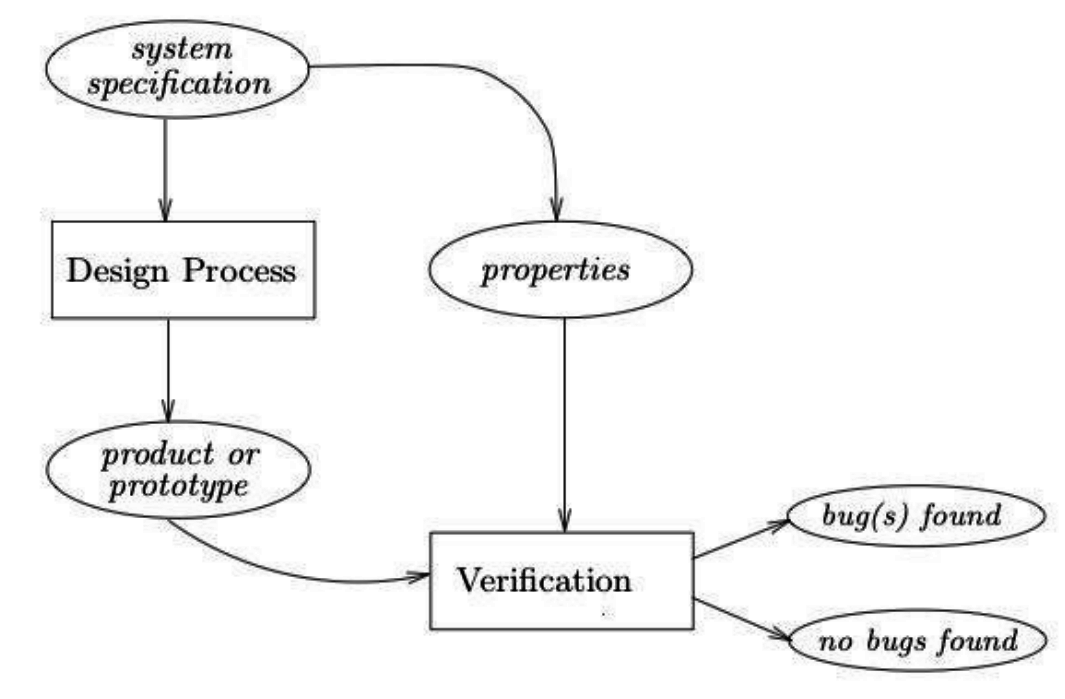
\includegraphics[scale=0.45]{img/Modello1.png}
\caption{Modello classico di ciclo di sviluppo del software.}
\label{fig:modello}
\end{center}
\end{figure}

In figura \ref{fig:modello} viene mostrato un approccio per la verifica di sistemi. Questo modello di ciclo di sviluppo del software presenta difetti importanti. La verifica del progetto viene fatta in fase avanzata dello sviluppo del codice. Modificare il codice sorgente nelle ultime fasi dello sviluppo potrebbe portare a numerosi problemi e rendere necessarie anche modifiche importanti. Inoltre, come mostrato in figura \ref{fig:costo_errori}, si può notare in quali fasi di sviluppo viene introdotto il maggior numero di errori e la loro incidenza sul loro costo di risoluzione. L'idea è quindi quella di trovare gli errori già nelle prime fasi del ciclo di sviluppo.

\begin{figure}[ht]
\begin{center}
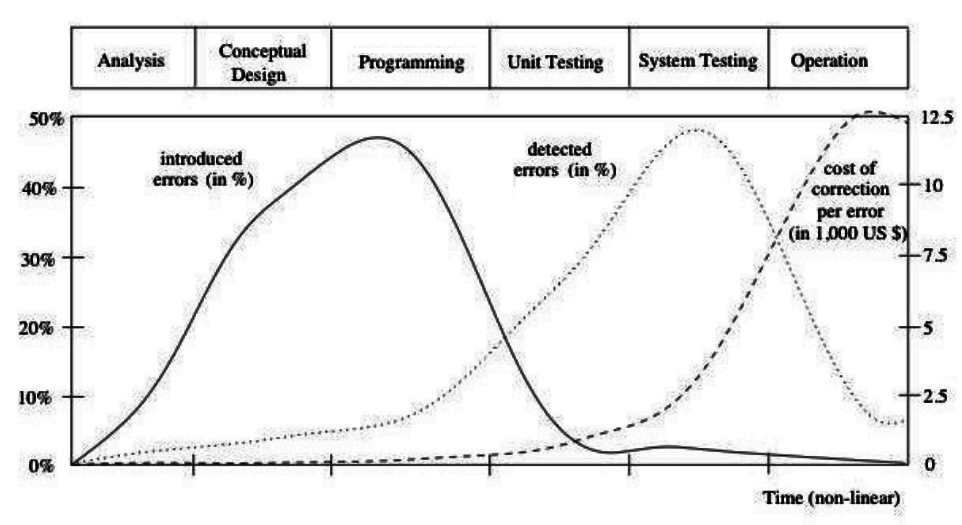
\includegraphics[scale=0.45]{img/costo_errori.png}
\caption{Grafico che mostra: introduzione degli errori, rilevazione degli errori e costo di correzione degli errori durante il ciclo di sviluppo del software.}
\label{fig:costo_errori}
\end{center}
\end{figure}
\section{Sistemi di transizione etichettati - (LTS)}
La verifica dei sistemi si serve di stumenti automatici. Quindi, viene naturale farsi la seguente domanda:

\begin{center}
\emph{come possiamo descrivere un sistema software?}
\end{center}

Ovviamente non possiamo utilizzare il linguaggio naturale, poichè esso è un linguaggio ambiguo. Abbiamo bisogno di un linguaggio formale che ci permetta di descrivere un sistema software senza ambiguità e che abbia una semantica ben definita. In altre parole abbiamo bisogno di un \emph{modello} del sistema. Per venire incontro a queste necessità sono stati ideati i sistemi di transizione etichettati, in inglese \emph{Label Transition System - (LTS)}. Gli LTS sono una generalizzazione degli \emph{automi a stati finiti - (FSM)} \cite{NoteProf}, infatti un LTS a differenza di un FSM ha le seguenti proprietà:

\begin{itemize}
 \item il numero degli stati di un LTS non è necessariamente finito;
 \item l'insieme delle transizioni di un LTS non è necessariamente finito.
\end{itemize}

\subsection{Definizione formale}
Un \emph{sistema di transizione etichettato} $TS$ è una sestupla 

\begin{equation}
TS\ =\ \langle\ S,\ Act,\ \rightarrow,\ I,\ AP,\ L\ \rangle
\end{equation}

\noindent dove:

\begin{itemize}
 \item $S\ $ è l'\emph{insieme degli stati} del sistema
 
 \item $Act\ $ è l'insieme finito dei simboli che rappresentano le \emph{azioni}. Le azioni possono essere di due tipi: \emph{interne} o \emph{esterne};
 
 \item $\rightarrow\ \subseteq S \times Act \times S\ $ è una relazione ternaria detta \emph{relazione di transizione} ed è un sottoinsieme del prodotto cartesiano $S \times Act \times S$.
 
 \textbf{Esempio:} $(p, \lambda, q) \in \rightarrow \ $ si può scrivere come $p\ \xrightarrow{\lambda}\ q$ e significa che il processo $p$ esegue l'azione $\lambda$ e si comporta come il processo $q$;
 
 \item $I\ \subseteq S $ è l'\emph{insieme degli stati iniziali};
 
 \item $AP\ $ è l'\emph{insieme delle proprietà atomiche}. Una proprietà è un predicato $P$ che associa ad ogni elemento $x$ o insieme $X$ un valore di verità;
 
 \item $L\ $ è la \emph{funzione di labeling} o sistema di etichettatura. È definita come
 \begin{equation}
  L:\ S \rightarrow 2^{AP}
 \end{equation}
 Il dominio della funzione $L$ è l'insieme degli stati del sistema $S$. Il codominio è l'insieme delle parti delle proprietà atomiche $AP$. Si ricorda che l'insieme delle parti o insieme potenza di un insieme $A$ è l'insieme
 \begin{equation}
  2^A=\ \{ X\ |\ X \subseteq A \}
 \end{equation}
 ovvero l'insieme di tutti i sottoinsiemi di $A$.
 Per ogni stato $s \in S$, l'insieme $L(s)$ è l'insieme di tutte le proposizione atimiche valide in $s$.
 
\end{itemize}

\subsubsection*{Esempio}

In figura \ref{fig:esempio-LTS} è mostrato il sistema di transizione $TS\ = \langle\ S,\ Act,\ \rightarrow , I, \dots \rangle$ di una macchina del caffè. Abbiamo che:

\begin{itemize}
 \item l'insieme degli stati del sistema:  S = \{ Ready,\ Select,\ Coffee,\ Tea \};
 \item l'insieme delle azioni:  Act = \{ Insert\_coin,\ Select\_coffee,\ Select\_tea,\ Supply\_coffee,\ Supply\_tea \};
 \item la relazione di transizione:
 
$ \rightarrow\ $= \{(Ready, Insert\_coin, Select),\ (Select, Select\_coffee, Coffee),\ (Select, Select\_tea, Tea),
 \  (Tea, Supply\_tea, Ready),\ (Coffee, Supply\_coffee, Ready)\}

\item l'insieme degli stati iniziali: I = \{ Ready \}
\end{itemize}


\begin{figure}[ht]

\begin{center}

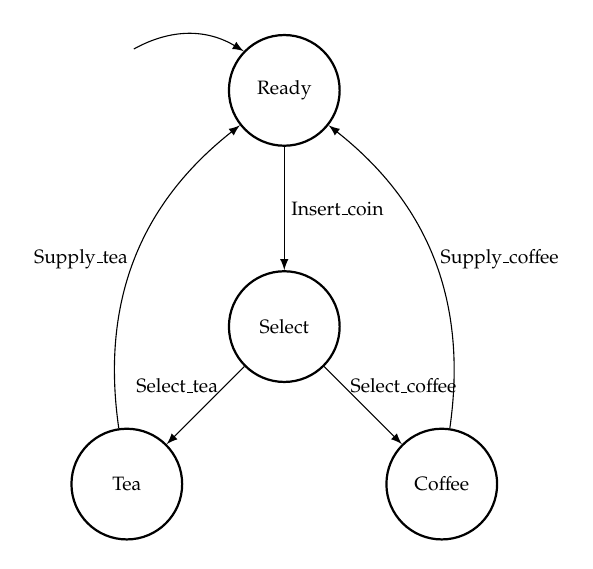
\begin{tikzpicture}

  \tikzstyle{node}=[shape=circle,inner sep=3pt, minimum size=40pt ,draw,thick]

  \tikzstyle{mpr}=[shape=circle,inner sep=1.5pt,draw,thick, fill=black]

  \tikzstyle{source}=[shape=rectangle,draw,dashed]

  \tikzstyle{lineDecorate}=[near start, -latex,draw]

  \tikzstyle{lineDecorateSource}=[-latex,draw,dashed, arrows=<->]

%[lineDecorate/.style={-,thick}, nodeDecorate/.style={shape=circle,inner sep=1.5pt,draw,thick}]

\scriptsize

%% nodes or vertices

\node (S) at (-2,5.5) {};

\node (A)[node] at (0,5) {Ready};

\node (B)[node] at (0,2) {Select};

\node (C)[node] at (-2,0) {Tea};

\node (D)[node] at (2,0) {Coffee};





%% edges or lines anchor=east

\path[->]

	(C) edge[lineDecorate, bend left] node[anchor=east, midway] {Supply\_tea} (A)

	(D) edge[lineDecorate, bend right] node[anchor=west, midway] {Supply\_coffee} (A)


;
%lineDecorateSource tratteggiata

\path[->]
	(S) edge[lineDecorate, bend left] node[anchor=west] {} (A)
	
	
	(A) edge[lineDecorate] node[anchor=west, midway] {Insert\_coin} (B)

	(B) edge[lineDecorate] node[anchor=west] {Select\_coffee} (D)

	(B) edge[lineDecorate] node[anchor=east] {Select\_tea} (C)

;
\end{tikzpicture}

\caption{Esempio di uno schema LTS per l'automa di una macchina del caffè.}

\label{fig:esempio-LTS}

\end{center}

\end{figure}




\subsection{Cammino o computazione}
In un LTS un \emph{cammino} ( o \emph{computazione}) $\pi$ è una sequenza finita (o infinita) della forma:

 \begin{equation}
  s_0 \lambda_0 s_1 \lambda_1 s_2 \lambda_2 \dots \dots \lambda_{n-1} s_n 
 \end{equation}
 
 \noindent dove $ \forall\ i,\ \exists\ s_i\ \xrightarrow{ \lambda_i }\ s_{i+1} \in\ \rightarrow\ $.
 
 Equivalentemente un cammino può essere scritto nelle seguenti forme:
 
 \begin{equation}
  (\ s_0,\ \lambda_0,\ s_1\ ), (\ s_1,\ \lambda_1,\ s_2\ ),\ \dots \dots, (\ s_{n-1},\ \lambda_{n-1},\ s_n\ )
 \end{equation}
 oppure
 \begin{equation}
  s_0\ \xrightarrow{ \lambda_0 }\ s_{1}\ \xrightarrow{ \lambda_1 }\ s_{2}\ \dots \dots \xrightarrow{ \lambda_{n-1} }\ s_{n}
 \end{equation}
 
\noindent Il cammino nullo è la sequenza vuota.
 \\
 
 Una cammino si dice \emph{iniziale} se $s_0\ \in I$.  
 Una cammino si dice \emph{massimale} se $s_n$ è uno stato terminale, oppure se è un cammino infinito.
 
 Uno stato $s\ \in\ S$ è \emph{raggiungibile} in un $TS\ =\ \langle\ S,\ Act,\ \rightarrow,\ I,\ AP,\ L\ \rangle$ se esiste un cammino finito ed iniziale tale che
 
  \begin{equation}
  s_0\ \xrightarrow{ \lambda_0 }\ s_{1}\ \xrightarrow{ \lambda_1 }\ s_{2}\ \dots \dots \xrightarrow{ \lambda_{n-1} }\ s_{n}\ =\ s
 \end{equation}
 
 Adesso consideriamo $TS\ = \langle\ S,\ Act,\ \rightarrow, \dots \rangle$. Indicheremo con:
 
 \begin{itemize}
  \item $\ Post( s, \lambda )\ = \{\ s' \in S\ |\ s\ \xrightarrow{ \lambda }\ s'\ \}\ $ ovvero l'insieme di tutti gli stati $s' \in S$ raggiungibili dallo stato $s \in S$ facendo un'azione $\lambda\ \in\ Act$;
  
  \item $\ Post(s) = \bigcup_{\lambda\ \in\ Act}^{} Post( s, \lambda )\ $ l'insieme di tutti gli stati raggiungibili dallo stato $s \in S,\ \forall \lambda \in Act$;
  
  \item $\ Preset( s, \lambda )\ = \{\ s' \in S\ |\ s'\ \xrightarrow{ \lambda }\ s\ \}\ $ l'insieme di tutti gli stati che attraverso un'azione $\lambda\ \in\ Act$ vanno nello stato $s \in S$;
  
  \item $\ Preset( s )\ = \bigcup_{\lambda\ \in\ Act}^{} Preset( s, \lambda )\ $ l'insieme di tutti gli stati che evolvono nello stato $s \in S,\ \forall \lambda \in Act$.
 \end{itemize}
 
\textbf{Stallo}

Un sistema si dice che è in \emph{stallo} (o in deadlock) quando non può eseguire nessuna azione e lo stato in cui si trova non è uno stato terminale.
\\
 
\textbf{Osservazioni:} un sistema è in stallo se $\ Post(s) = \emptyset $. Inoltre, se $s \in S$ è uno stato terminale, allora $\ Post(s) = \emptyset $.
\\

\clearpage

\subsection{Determinismo e non determinismo}
Un sistema si dice \emph{non deterministico} se può comportarsi in due o più modi differenti con lo stesso input. In formule:

\begin{equation}
 \exists \, (s, \lambda)\ :\ \rvert Post( s, \lambda ) \rvert > 1
\end{equation}

Un sistema si dice \emph{deterministico} se per ogni stato del sistema, esiste una e una sola azione tale che è possibile determinare in modo univoco lo stato successivo. In formule:

\begin{equation}
 \forall s \in S,\ \exists! \, \lambda \in Act\ :\ \rvert Post( s, \lambda ) \rvert = 1
\end{equation}

Si possono avere due tipi di determinismo:

\begin{itemize}
 \item Action Determinism
 \item AP-Determinism
\end{itemize}

Un sistema è \emph{action deterministic} (deterministico rispetto alle azioni) allora
\begin{equation}
|I| \leq 1,\ \forall s \in S,\ \forall \lambda \in Act\ \Leftrightarrow\ \rvert Post( s, \lambda ) \rvert \leq 1
\end{equation}
ovvero, l'insieme degli stati iniziali deve avere cardinalità al più uno e per ogni coppia stato-azione, l'insieme degli stati successivi deve avere cardinalità al più uno.

Un sistema è \emph{AP-deterministic} (deterministico rispetto alle proprietà atomiche) allora
\begin{equation}
 |I| \leq 1,\ \forall s \in S,\ \forall \lambda \in Act\ \Leftrightarrow\ \rvert Post(s) \cap \{ s' \in S\ |\ L(s') = A \} \rvert \leq 1
\end{equation}
ovvero, l'insieme di tutti gli stati successivi allo stato $s$ intersecato con l'insieme degli stati che soddisfano la proprietà atomica $A$ ha cardinalità al più $1$.



 


 

\section{Action-based Computation Tree Logic - (aCTL)}
Abbiamo visto che un sistema può essere modellato per mezzo dei sistemi di transizione etichettati (o LTS). Adesso, abbiamo bisogno di un linguaggio formale che ci permetta di scrivere in modo non ambiguo le proprietà del sistema.

\subsection{Logiche temporali}
Esistono diversi tipi di logiche, tra cui le più note sono la logica modale e la logica temporale. La logica modale permette di esprimere proprietà locali di uno stato. Ad esempio: \emph{``Andrea e Marco sono felici?''}. Il limite di questa logica è che non possiamo sapere se Andrea e Marco continueranno ad essere felici. Questo limite può essere superato attraverso l'utilizzo di logiche temporali.

Le logiche temporali possono essere di due tipi:

\begin{itemize}
 \item logiche temporali lineari;
 \item logiche temporali branching.
\end{itemize}

\noindent Nel seguito parleremo di aCTL che è una logica temporale di tipo branching \cite{NoteProf}.

\subsection{Logica aCTL}
aCTL sta per Action-based Computation Tree Logic. È una logica temporale di tipo branching, ovvero il tempo è modellato con una struttura ad albero e quindi l'evoluzione futura non è determinata in modo univoco. Questo approccio si avvicina alla vera esecuzione di un programma in cui alcune scelte vengono fatte durante l'esecuzione del processo.
Le formule di aCTL si riferiscono esplicitamene alle azioni che il sistema può fare.

\clearpage
\subsubsection{Sintassi di aCTL}
Distinguiamo due categorie sintattiche:

\begin{itemize}
 \item \emph{state formule} $\ \phi$;
 \item \emph{path formule} $\ \varphi$:
\end{itemize}

\noindent Il linguaggio è generato dalla seguente grammatica:
\\

%\begin{center}
\textbf{{State-formula}}
%\end{center}

\begin{equation}
 \phi ::= true\ |\ \neg \phi\ |\ AP\ |\ \phi_1 \ \wedge \phi_2\ |\ \exists\varphi\ |\ \forall\varphi
\end{equation}

\begin{itemize}
 \item $true\ $: è l'assioma \emph{vero};
 
 \item $AP\ $: sono le proposizioni atomiche. Ad esempio: la state formula $\phi = a$ è vera per lo stato $\ s\ $ se $\ a \in L(s) \subseteq AP$;
 
 \item $\neg \phi\ $: è la negazione di $\phi$;
 
 \item $\phi_1 \wedge \phi_2\ $: è la congiunzione di $\phi_1$ e $ \phi_2\ $;
 
 \item $\exists\varphi\ $: è il quantificatore esistenziale. Il suo significato è che esiste almeno un cammino (o computazione) che partendo dallo stato attuale permette di raggiungere uno stato che soddisfa $\varphi$;
 
 \item $\forall\varphi\ $: è il quantificatore universale. Il suo significato è che tutti i cammini che partono dallo stato corrente soddisfano la proprietà $\varphi$.
\end{itemize}


%\begin{center}
\textbf{{Path-formula}}
%\end{center}

\begin{equation}
 \varphi ::= X_A \phi\ |\ \phi\ {}_{A}\mathcal{U}\ \psi\ |\ \phi\ {}_{A}\mathcal{U}_B\ \psi
\end{equation}

\begin{itemize}
 \item $X_A \phi\ $: è l'operatore \emph{next} associato all'azione $A$. La formula è soddisfatta se a partire dallo stato corrente è possibile fare un'azione $A$ ed andare in uno stato che soddisfa la proprietà $\ \phi$;
 
 \item $\phi\ {}_{A}\mathcal{U}\ \psi\ $: è l'operatore \emph{until} associato all'azione $\ A$. La formula è soddisfatta se si percorre un cammino (anche nullo) eseguendo azioni in $\ A$ e tutti gli stati soddisfano la proprietà $\ \phi$ fino a quando non si arriva in uno stato che soddisfa la proprietà $\ \psi$;
 
 \item $\phi\ {}_{A}\mathcal{U}_B\ \psi\ $: è loperatore \emph{until} associato all'azione $\ A$ e $\ B$. La formula è soddisfatta se si percorre un cammino (anche nullo) eseguendo azioni in $\ A$ e tutti gli stati soddisfano la proprietà $\ \phi$ fino a quando non si arriva in uno stato che soddisfa la proprietà $\ \psi$ attraverso l'esecuzione di una azione in $\ B$.
\end{itemize}

Le formule aCTL sono interpretate sui sistemi di transizione etichettati. In particolare è bene fare una distinzione tra le state formule e path formule. Le state formule sono valutate sugli stati del LTS, viceversa le path formule sono valutate sui cammini o computazioni del LTS.
Come si può notare, una path formula può occorrere in una state formula come parametro degli operatori $\exists\ $ e $\forall\ $.


Esistono altri operatori, detti operatori derivati, che permettono di riscrivere le formule in altre formule equivalenti che possono risultare più comprensibili.

\begin{alignat}{4}
false\  & \equiv\ \neg true \\
\phi_1 \wedge \phi_2\ & \equiv\ \neg\ ( \neg\phi_1 \vee \neg\phi_2 ) \\
\phi_1 \Rightarrow \phi_2\ & \equiv\ \neg\phi_1 \vee \phi_2\ \\
\phi_1 \Leftrightarrow \phi_2\ & \equiv\ (\phi_1 \Rightarrow \phi_2) \wedge\ (\phi_2 \Rightarrow \phi_1)  
\end{alignat}


\clearpage
\subsubsection{Operatori}
Diamo ora una classificazione degli operatori. Gli operatori possono essere di due tipi: logici e temporali.
\\

\textbf{Operatori logici}

Gli operatori logici sono i seguenti:

\begin{equation}
  \neg,\ \wedge,\ \vee,\ \Rightarrow,\ \Leftrightarrow
\end{equation}


\textbf{Operatori temporali}

Gli operatori temporali sono

\begin{equation}
  \forall,\ \exists,\ X,\ U,\ \Diamond,\ \Box
\end{equation}



in particolare gli operatori $\exists\ $ e $\forall\ $ sono dei quantificatori di cammino.

\subsubsection{Semantica}

Come anticipato le formule aCTL sono interpretate sui sistemi di transizione etichettati. Un sistema di transizioni, come abbiamo visto, è una sestupla $TS\ =\ \langle\ S,\ Act,\ \rightarrow,\ I,\ AP,\ L\ \rangle$ dove $S$ è l'insieme degli stati, Act è l'insieme dei simboli che rappresentano le azioni, $\rightarrow$ è l'insieme delle relazioni di transizione, I è l'insieme degli stati iniziali, AP è l'insieme delle proprietà atomiche e L è la funzione di labeling.

Sia quindi TS tale sistema di transizioni con s $\in$ S e $\Phi \in F$ dove F è l'insieme delle formule aCTL.
La semantica di una formula temporale è definita dalla  soddisfazione della seguente relazione:

\begin{equation}
	\models : ( TS \; \times \; S \; \times \; F ) \rightarrow \lbrace true, false \rbrace
\end{equation}

\clearpage
Una proposizione atomica è vera (\emph{true}) in uno stato $s_i$ quando:

\begin{equation}
TS, s_i \models p \; \text{se e solo se}\; p \in L(s_i)
\end{equation}


La relazione di implicazione semantica può essere definita per induzione strutturale su $\Phi$.

\begin{alignat}{4}
TS, s_i \models & \; true \; 			&& \quad  && 				\forall  s \in S \\
TS, s_i \models & \; \neg \Phi  			&& \quad \Leftrightarrow \quad &&	\neg TS, s_i  \models \Phi \\
TS, s_i \models & \; \Phi \wedge \Psi 		&&\quad \Leftrightarrow \quad && 	TS, s_i \models \Phi \text{ and } TS , s_i \models \Psi \\
TS, s_i \models & \; \Phi \vee \Psi  		&&\quad \Leftrightarrow \quad &&	TS, s_i \models \Phi \text{ or } TS , s_i \models \Psi \\
TS, s_i \models & \; \Phi \Rightarrow \Psi  	&&\quad \Leftrightarrow \quad && (\neg TS, s_i \models \Phi \text{ or } TS , s_i \models \Psi ) \\
TS, s_i \models & \; \Phi \Leftrightarrow \Psi  	&& \quad \Leftrightarrow \quad 	& \begin{split} &( TS, s_i \models \Phi \text{ or } TS , s_i \models \Psi ) \\ & \vee (\neg TS, s_i \models \Phi \text{ or } \neg TS , s_i \models \Psi )\end{split} 
\end{alignat}

Gli operatori temporali, considerando $\pi = (s_0, s_1, \dots, s_n) \in Path(s)$ un generico cammino avente origine dallo stato $s_i \in S$, hanno la seguente semantica:

\begin{alignat}{4}
TS, s_i \models & \; \forall \;  \varphi 					&& \quad \Leftrightarrow \quad &&  	\forall \pi \in Path(s_i):  \pi \models \varphi  \\
TS, s_i \models & \; \exists \;  \varphi					&& \quad \Leftrightarrow \quad &&	\exists \pi \in Path(s_i):  \pi \models \varphi
\end{alignat}

\clearpage
Rimane infine da definire la semantica per gli operatori di $\chi$ e di $\mathcal{U}$ lungo un cammino $\pi $:

\begin{alignat}{4}
\pi = s_0 \alpha_0 s_1 \dots  \models & \; \chi_A \; \Phi 								&& \quad \Leftrightarrow \quad &&  	\alpha_0 \in A \text{ and } TS,s_1 \models \Phi \\
\pi =  s_0 \alpha_0 s_1 	 \dots \alpha_{n-1} s_n \models & \; \Phi_A \; \mathcal{U} \;  \Psi		&& \quad \Leftrightarrow \quad & \begin{split} & \exists j \ge 0: \; \pi(j) \models \Psi \text{ and } \\ &  \forall 0 \le i < j:  \; \pi(i) \models \Phi \text{ and }  \alpha_i \in A )\end{split} \\
\pi =  s_0 \alpha_0 s_1 	 \dots \alpha_{n-1} s_n \models & \; \Phi_A \; \mathcal{U}_B \;  \Psi	&& \quad \Leftrightarrow \quad & \begin{split} & \exists j \ge 1: \; \pi(j) \models \Psi \text{ and } \alpha_{j-1} \in B \\ &  \forall 0 \le i < j:  \; \pi(i) \models \Phi \text{ and } \\ &  \forall 0 \le i < j-1 \; \alpha_i \in A \end{split} 
\end{alignat}

In base a quanto è stato appena enunciato è facile verificare anche le formule 
\begin{alignat}{4}
TS, s_i \models & \; \forall \; \Box \; \Phi \\
TS, s_i \models & \; \exists \; \Box \; \Phi \\
TS, s_i \models  & \; \forall \; \Diamond \; \Phi \\
TS, s_i \models & \; \exists \; \Diamond	\; \Phi	 
%TS, s_i \models & \; \forall \; [\Phi_1 \; \mathcal{U} \; \Phi_2]
\end{alignat}

Queste formule sono infatti sono facilmente ricavabili nel modo seguente:

\begin{alignat}{4}
\exists\ \Diamond_A \phi\ 			&\equiv\ \exists\ (true\ {}_{A}\mathcal{U}\ \phi ) \\ 
\forall\ \Diamond_A \phi\ 			&\equiv\ \forall\ (true\ {}_{A}\mathcal{U}\ \phi ) \\
\exists\ \Box_A \phi\			&\equiv\ \neg\ \forall\ \Diamond_A\ \neg\ \phi \\
\forall\ \Box_A \phi\ 			&\equiv\ \neg\ \exists\ \Diamond_A\ \neg\ \phi  \\
\forall [ \Phi \; \mathcal{U} \; \Psi ] 	&\equiv \neg \exists \Box \neg \Psi \wedge \neg \exists (\neg \Psi \mathcal{U} (\neg \Phi \wedge \neg \Psi))
\end{alignat}
\section{Model checking}
Il \emph{model checking} è un metodo per la verifica dei sistemi. Fu introdotto da E. Clarke, A. Emerson e J. Sifakis con cui si aggiudicarono nel 2007 il A.M. Turing Award.
Il metodo del model checking è schematizzato in figura \ref{fig:model_checking}. Un \emph{model checker} riceve in \emph{input} il modello del sistema software ed i requisiti che deve soddisfare. In \emph{ouput} restituirà un valore booleano: \emph{true} o \emph{false} nel caso in cui la proprietà che si è andata a verificare  sia rispettivamente soddisfatta o non soddisfatta. Se la proprietà non è soddisfatta viene fornito un \emph{controesempio}.
\\

\begin{figure}[ht]
\begin{center}
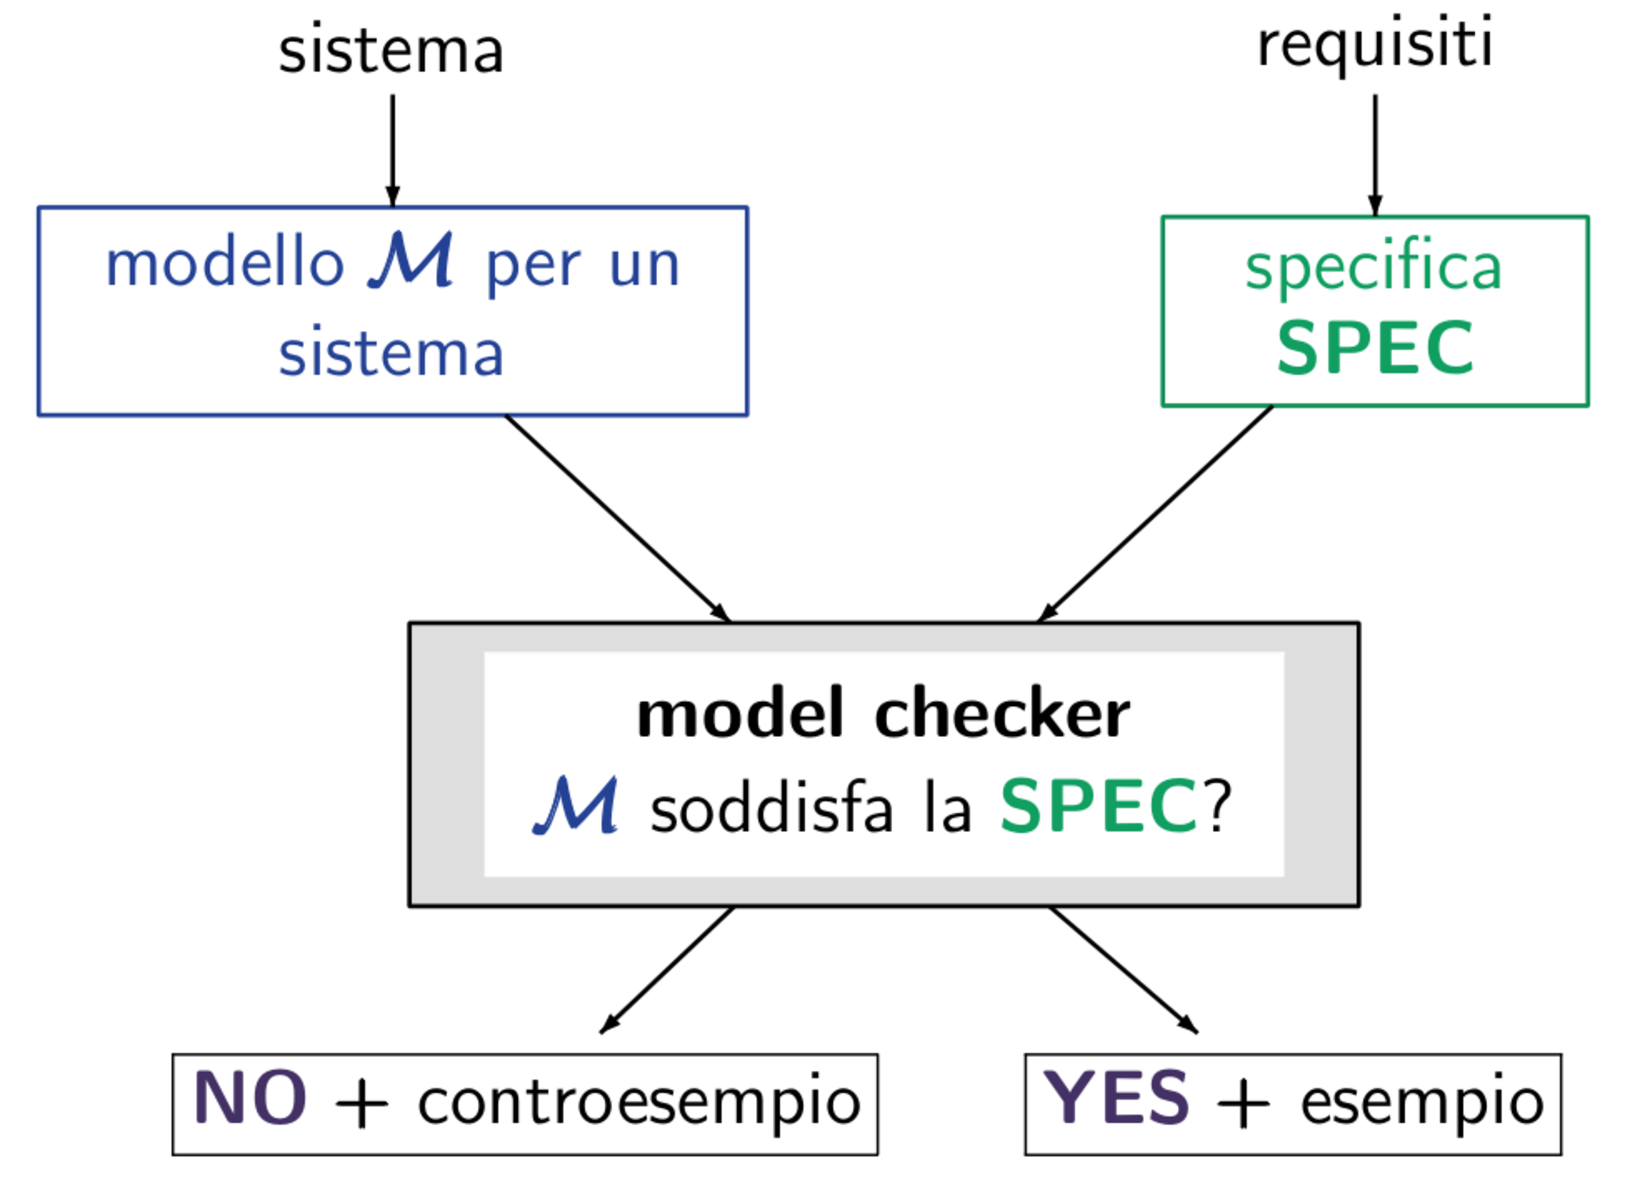
\includegraphics[scale=0.3]{img/Model-checking.pdf}
\caption{Model checking.}
\label{fig:model_checking}
\end{center}
\end{figure}

Formalmente, la verifica di una proprietà tramite model checking consiste: dato un modello del sistema $M$ con stato iniziale $s$ e data una proprietà $\phi$ che il sistema deve soddisfare, fare il model checking consiste nel dire se:

\begin{alignat}{4}
M,\ s 		& 	\models \phi \\
M,\ s  		& 	\not \models \phi
\end{alignat}

Il modello del sistema su cui vogliamo fare model checking è descritto mediante un sistema di transizione etichettato (LTS). Le proprietà da verificare sono descritte attraverso un linguaggio formale in logica temporale, nel nostro caso aCTL.

\subsection{Model checking globale e locale}

Come abbiamo detto i sistemi sono una composizione di più modelli che descrivono il comportamento di un processo. Un limite del model checking è il cosidetto fenomeno dell'\emph{esplosione dello spazio degli stati}. La rappresentazione di un sistema con un numero elevato di stati (ad esempio dell'ordine di $10^{100}$) richiede molta memoria. 

Possiamo distinguere due approcci di model checking:
\begin{itemize}
 \item model checking globale
 \item model checking locale
\end{itemize}

Il \emph{model checking globale}, consiste nell'andare a verificare se tutti gli stati del sistema preso in considerazione, verificano una proprietà. Questa è un'operazione computazionalmente onerosa in quanto verrà generato l'intero spazio degli stati. Inoltre, vengono generati anche gli stati che non sono rilevanti al fine di dimostrare la soddisfacibilità della formula. 
L'approccio utilizzato è quello di una ricerca \textit{bottom-up} a partire dalle foglie dell'albero fino a risalire alla radice.

Viceversa, il \emph{model checking locale} genera solo gli stati che servono effettivamente a verificare la proprietà. In questo caso viene adottato un approccio \textit{top-down}, e cioè a partire da un nodo radice si percorre l'albero verso le foglie.

\clearpage
\subsubsection{Existential normal form (ENF)}

Al fine di sviluppare un model checker, viene utilizzata una notazione alternativa alle formule aCTL, l'Existential Normal Form (ENF), che permette una più semplice trasposizione in forma algoritmica.
Qualsiasi formula aCTL può essere infatti scritta come combinazione delle formule ENF.

\begin{equation}
\Phi ::= true \; | \; ap \; | \; \Phi_1 \wedge \Phi_2 |  \neg \Phi | \exists \; \chi_A \; \Phi \; | \; \exists ({\Phi_1}_A \; \mathcal{U}\; \Phi_2) \; | \; \exists ({\Phi_1}_A \; \mathcal{U}_B \; \Phi_2) \; | \; \exists \Box_A \Phi
\end{equation}

I passi da eseguire per verificare se uno stato, appartenente a TS,  verifica una formula aCTL $\hat{\Phi}$, sono i seguenti:

\begin{enumerate}
\item si converte la formula $\hat{\Phi}$ nella sua equivalente $\Phi$ in ENF
\item si calcola ricorsivamente l'insieme $ Sat(\Phi) = \lbrace s \in S | s \models \Phi \rbrace $
\item TS, $s_i \; \models \Phi $ se e solo se $ s_i \in Sat(\Phi) $
\end{enumerate}

\clearpage

Definiamo quindi per casi, i possibili valori assumibili da Sat($\Phi$):

\begin{alignat}{4}
Sat(true)					&\quad 	\rightarrow	\quad&&	S 	\\
Sat(ap)					&\quad	 \rightarrow	\quad&&	\lbrace s | ap \in L(s) \rbrace 	\\
Sat(\Phi \wedge \Psi)			&\quad	 \rightarrow	\quad&&	Sat(\Phi) \cap Sat(\Psi)  	\\
Sat(\neg \Phi)				&\quad	 \rightarrow	\quad&&	S \ Sat(\Phi) 	\\
Sat(\exists \mathcal{X}_A \Phi)		&\quad	 \rightarrow	\quad&&	\lbrace s | Post_A(s) \cap Sat(\Phi) \neq \emptyset 	\\
Sat(\exists \Phi_A \mathcal{U} \Psi)	&\quad	 \rightarrow	\quad&	\begin{split} & \text{il più piccolo sottoinsieme T} \subseteq \text{S,tale che:} 	\\
														& 1)\; Sat(\Psi) \subseteq T  \\
														& 2)\; se \;s \in Sat(\Phi) \wedge Post_A(s) \cap T \neq \emptyset \Rightarrow s \in T
												\end{split} \\
Sat(\exists \Phi_A \mathcal{U}_B \Psi)	&\quad	 \rightarrow	\quad&	\begin{split} & \text{il più piccolo sottoinsieme T} \subseteq \text{S,tale che:} 	\\
														& 1)\; se \; s \in Sat(\Phi) \wedge Post_B(s) \cap Sat(\Psi) \neq \emptyset \Rightarrow s \in T \\
														& 2)\; se \; s \in Sat(\Phi) \wedge Post_A(s) \cap T \neq \emptyset \Rightarrow s \in T
												\end{split} \\
Sat(\exists \Box_A \Phi)			&\quad	 \rightarrow	\quad&	\begin{split} & \text{il più piccolo sottoinsieme T} \subseteq \text{S,tale che:} 	\\
														& 1)\; Sat(\Psi) \subseteq T  \\
														& 2)\; se \; s \in T \Rightarrow Post_A(s) \cap T \neq \emptyset 
												\end{split}
\end{alignat}




\section{Algoritmi}

L'obiettivo del model checking locale per aCTL è il seguente: data una struttura $\mathcal{T}$ e una formula aCTL \emph{f},  determinare se $\mathcal{T}$ soddisfa \emph{f}.
Verrà adesso introdotta l'implementazione di un algoritmo per la risoluzione del problema.
\\

\noindent L'algoritmo dovrà soddisfare le seguenti specifiche:
\begin{itemize}
\item input: un LTS $\mathcal{T}$, uno stato $s$, una formula CTL $f$;
\item output: true $ \Leftrightarrow \; \mathcal{T}$, $s$ $\models$ $f$.
\end{itemize}
L'algoritmo dovrà inoltre operare secondo una modalità \textit{goal-oriented}, e cioè con approccio top-down, per decidere se $\mathcal{T}$, $s$ $\models$ $f$. Gli stati che dovranno essere controllati durante la sua esecuzione dovranno essere quindi solo quelli strettamente necessari a raggiungere lo stato di goal.


Per poter eseguire l'algoritmo nel minor tempo possibile si è reso necessario l'utilizzo di una variabile globale per tenere traccia di tutte le informazioni raccolte durante l'esecuzione.
Questa struttura è stata definita nel modo seguente:

\begin{equation}
info: S \; x \; sub(f) \rightarrow \lbrace 0, 1, \bullet \rbrace,
\end{equation}

dove $sub(f)$ rappresenta l'insieme delle sottoformule di $f$.
I valori assumibili dalla variabile rappresentano la soddisfacibilità di una determinata formula.
Se uno stato $s$ $\in$ S non soddisfa la formula $f$, si avrà di conseguenza che \mbox{info($s$, $f$) = 0}. Nel caso in cui $s$ soddisfi la formula $f$ si avrà che \mbox{info($s$, $f$) = 1}, mentre nel caso in cui non sia ancora stato possibile determinarlo si avrà  \mbox{info($s$, $f$) = $\bullet$}.

Formalmente il significato della variabile info è dato dalla seguente invariante che dovrà essere sempre valida durante l'esecuzione dell'algoritmo:

\begin{equation}
I \stackrel{def}{=} \forall s,f: \; (info(s, f) = 0 \Rightarrow \mathcal{T}, s \nvDash  f)  \wedge (info(s, f) = 1  \Rightarrow \mathcal{T},s \models f)
\end{equation}

Viene mostrato in seguito il codice relativo allo schema generale dell'algoritmo:
\\

\begin{lstlisting}[mathescape, caption= Schema generale dell'algoritmo, label=check]
Check(s, $\Phi$) $\lbrace$	
	if info(s, $\Phi$) $\neq \bullet$
		return;	
	switch($\Phi$) $\lbrace	$
		case a: 
			if s $\in \mathbb{L}$(p) then
				info(s, $\Phi$) := 1;
			else
				info(s, $\Phi$) := 0;
		case $\neg \; \Phi'$:
			Check(s, $\Phi'$);
			info(s, $\neg \; \Phi'$) = $\neg$ info(s, $\Phi'$);
		case $\Phi_1 \wedge \Phi_2$:
			Check(s, $\Phi_1$);
			if info(s, $\Phi_1$) = 0 then
				info(s, $\Phi_1 \wedge \Phi_2$) = 0;
			else $\lbrace$
				Check(s, $\Phi_2$);
				info(s, $\Phi_1 \wedge \Phi_2$) = info(s, $\Phi_2$);
			$\rbrace$
		case $\exists\chi_A\Phi'$:
			foreach $s' \in \lbrace s' | \exists \alpha \in A: s  \xrightarrow{ \alpha } s' \rbrace \lbrace$
				Check($s', \Phi'$);
				if (info($s', \Phi'$)==1) $\lbrace$
					info($s', \exists\chi_A\Phi'$) = 1;
					return;
				$\rbrace$
			$\rbrace$
			info(s, $\exists\chi_A\Phi'$) = 0;
		case $\forall \chi_A\Phi'$:
			init(s) = $\lbrace \alpha | \exists s': s\xrightarrow{\alpha} s' \rbrace$
			if ( init(s) $\nsubseteq$ A ) then $\lbrace$
				info(s, $\forall \chi_A\Phi'$) = 0;
				return;
			$\rbrace$
			foreach $s' \in \lbrace s' | \exists \alpha \in A: s  \xrightarrow{ \alpha } s' \rbrace \lbrace$
				Check($s', \Phi'$);
				if (info($s', \Phi'$)==0) then $\lbrace$
					info($s', \exists\chi_A\Phi'$) = 0;
					return;
				$\rbrace$
			$\rbrace$
			info(s, $\exists\chi_A\Phi'$) = 1;
		case $\exists{\Phi_1}_A \mathcal{U} \Phi_2$:
			CheckEU(s, A, $\Phi_1, \Phi_2$);
		case $\forall{\Phi_1}_A \mathcal{U} \Phi_2$:
			CheckAU(s, A, $\Phi_1, \Phi_2$);
	$\rbrace$
$\rbrace$
\end{lstlisting}

L'implementazione in Code \ref{check}, affronta in modo ricorsivo tutte le formule previste dalla sintassi da aCTL.
Nel caso delle proprietà $\exists{\Phi_1}_A \mathcal{U} \Phi_2$ e $\forall{\Phi_1}_A \mathcal{U} \Phi_2$, l'implementazione è stata suddivisa nelle funzioni dedicate CheckEU e CheckAU.
\\

\begin{lstlisting}[mathescape, caption=Implementazione di CheckEU]
CheckEU(s, A, $\Phi_1$, $\Phi_2$) $\lbrace$
	V = $\emptyset$; 							// stati visitati
	E = $\lbrace s \rbrace$; 							// stati in corso di visita
	goal = $\bullet$;
	while (goal == $\bullet \; \wedge \; E \neq \emptyset $) $\lbrace$
		s'= pick(E);
		E = E \ $\lbrace$s'$\rbrace$;
		V = V $\cup$ $\lbrace$s'$\rbrace$;
		Check(s', $\Phi_2$);
		if (info(s', $\Phi_2$) == 1) then $\lbrace$
			goal = s';
			break;
		$\rbrace$
		Check(s', $\Phi_1$);
		if (info(s', $\Phi_1$) == 1) then $\lbrace$
			E = E $\cup \; \lbrace$s'' | $\exists \; \alpha \in A: s' \xrightarrow{\alpha}s'' \rbrace$ \ V;
		$\rbrace$	
	$\rbrace$
	if (goal $\neq \; \bullet$) then
		info(s, $\exists{\Phi_1}_A \mathcal{U} \Phi_2$) = 1;
	else
		info(s, $\exists{\Phi_1}_A \mathcal{U} \Phi_2$) = 0;
$\rbrace$
\end{lstlisting}

Il codice precedente esegue una visita (parziale) in profondità dalla radice $s$. La ricerca viene interrotta appena viene trovato uno stato $s$ che soddisfa $\exists{\Phi_1}_A \mathcal{U} \Phi_2$, e cioè quando info($s$, $\exists{\Phi_1}_A \mathcal{U} \Phi_2$) = 1, oppure quando viene trovato uno stato s che soddisfa $\Phi_2$. Se info($s$, $\exists{\Phi_1}_A \mathcal{U} \Phi_2$) = 0, oppure se sia $\Phi_1$ che $\Phi_2$ non sono soddisfatti da uno stato s, allora non è necessario proseguire.
Al fine di implementare un ricerca in profondità, la struttura E mantiene traccia degli stati in corso di visita e viene gestita in modalità LIFO.


Ignorando il tempo richiesto per processare le chiamate alla funzione di Check, possiamo osservare che il tempo di esecuzione di CheckEU è di $\mathcal{O}(|\mathcal{T}|)$. Per questo motivo nel caso in cui si abbiano più formule annidate del tipo $\exists[\mathcal{\_U\_}]$ non è possibile effettuare model checking in tempo lineare. 

Consideriamo per esempio la formula $\exists{f_1}_A \mathcal{U} f_2$ dove $f_1$ e $f_2$ contengono a loro volta sottoformule del tipo $\exists[\mathcal{\_U\_}]$. Per decidere se $\mathcal{T}, s \models \exists{f_1}_A \mathcal{U} f_2$, nel caso peggiore potrebbe essere necessario controllare $f_1$ e $f_2$ per ogni stato e ognuna di queste ricerche potrebbe richiedere un attraversamento completo del sistema di transizioni impiegando un tempo quadratico\cite{ALMC}.

Per poter migliorare le performance di CheckEU è necessario provvedere  a memorizzare nella struttura	 di info maggiori informazioni sulla propietà in esame. Nell'implementazione precedente infatti la struttura di info veniva aggiornata solamente per lo stato di s. La funzione può essere quindi modificata per salvare informazioni sulla validità della proprietà per tutti gli stati visitati durante l'esecuzione di CheckEU.
Una possibile modifica di CheckEU viene mostrata in seguito.
\\
\begin{lstlisting}[mathescape, caption=Implementazione modificata di CheckEU]
CheckEU(s, A, $\Phi_1$, $\Phi_2$) $\lbrace$
	V = $\emptyset$; 							// stati visitati
	E = $\lbrace s \rbrace$; 							// stati in corso di visita
	goal = $\bullet$;
	while (goal == $\bullet \; \wedge \; E \neq \emptyset $) $\lbrace$
		s'= pick(E);
		E = E \ $\lbrace$s'$\rbrace$;
		V = V $\cup$ $\lbrace$s'$\rbrace$;
		Check(s', $\Phi_2$);
		if (info(s', $\Phi_2$) == 1) then $\lbrace$
			goal = s';
			break;
		$\rbrace$
		Check(s', $\Phi_1$);
		if (info(s', $\Phi_1$) == 1) then $\lbrace$
			E = E $\cup \; \lbrace$s'' | $\exists \; \alpha \in A: s' \xrightarrow{\alpha}s'' \rbrace$ \ V;
		$\rbrace$	
	$\rbrace$
	if (goal == $\bullet$) then $\lbrace$
		foreach s' $\in$ V										
			info(s, $\exists{\Phi_1}_A \mathcal{U} \Phi_2$) = 0;
	$\rbrace$ else	$\lbrace$								
		foreach s' in $\in$ V $\lbrace$
			if s $\stackrel{*}{\rightsquigarrow}$ goal then
				info(s, $\exists{\Phi_1}_A \mathcal{U} \Phi_2$) = 1;
			else
				info(s, $\exists{\Phi_1}_A \mathcal{U} \Phi_2$) = 0;
		$\rbrace$
	$\rbrace$
$\rbrace$
\end{lstlisting}

La parte terminale della funzione è stata modificata per aggiornare tutti i nodi visitati durante l'esecuzione dell'algoritmo.
Se al termine di CheckEU la variabile di goal è ancora uguale a $\bullet$, significa che nessun cammino soddisfa la proprietà in esame. Se invece la variabile di goal è stata modificata, significa che conterrà al suo interno lo stato terminale del cammino che soddisfa la proprietà. Indicando con  s $\stackrel{*}{\rightsquigarrow}$ goal il cammino dallo stato di partenza a quello di goal, si aggiorna lungo il cammino la variabile info(s, $\exists{\Phi_1}_A \mathcal{U} \Phi_2$) = 1, ponendola pari a 0 per tutti gli stati che non ne fanno parte.
Il cammino può essere ricavato risalendo all'indietro dallo stato di goal qualora vengano memorizzate anche le transizioni inverse.
Un metodo alternativo alla memorizzazione delle transizioni inverse è quello proposto da Vegauwen e Lewi \cite{ALMC} che incorpora il calcolo del cammino all'interno della ricerca depth-first.

L'implementazione della funzione di CheckAU è molto più semplice di quella di CheckEU. Infatti nel caso in cui, durante una ricerca depth-first, venga trovato un cammino ciclico che soddisfa $\Phi_1$ ma non $\Phi_2$ possiamo concludere che la formula $\forall{\Phi_1}_A \mathcal{U} \Phi_2$ è falsa per tutti gli stati analizzati.
\\
\begin{lstlisting}[mathescape, caption=Implementazione di CheckAU]
CheckAU(s, A, $\Phi_1$, $\Phi_2$) $\lbrace$
	V = $\emptyset$; 							// stati visitati
	E = $\lbrace s \rbrace$; 							// stati in corso di visita
	goal = $\bullet$;
	while (goal == $\bullet \; \wedge \; E \neq \emptyset $) $\lbrace$
		s'= pick(E);
		E = E \ $\lbrace$s'$\rbrace$;
		V = V $\cup$ $\lbrace$s'$\rbrace$;
		Check(s', $\Phi_2$);
		// se info = 1, il ramo e' verificato
		if (info(s', $\Phi_2$) == 0) then $\lbrace$
			Check(s', $\Phi_1$);
			if (info(s', $\Phi_1$) == 0) then $\lbrace$
				goal = 0;
				break;							// esce dal ciclo
			$\rbrace$ else $\lbrace$
				int(s') = $\lbrace \; \alpha \; |\; \exists\; s' \xrightarrow{\alpha}s'' \rbrace$;
				if (int(s') $\nsubseteq$ A) $\lbrace$
					goal = 0;
					break;						// esce dal ciclo
				$\rbrace$
				E = E $\cup \; \lbrace$s'' | $\exists \; \alpha \in A: s' \xrightarrow{\alpha}s'' \rbrace$ \ V;
			$\rbrace$	
		$\rbrace$
	$\rbrace$
	if (goal == 0) then
		info(s, $\forall{\Phi_1}_A \mathcal{U} \Phi_2$) = 0;
	else
		info(s, $\forall{\Phi_1}_A \mathcal{U} \Phi_2$) = 1;
$\rbrace$
\end{lstlisting}

Nel caso in cui si voglia salvare le informazioni ricavate su tutti i nodi visitati è sufficiente modificare la funzione nel modo seguente.
\\
\begin{lstlisting}[mathescape]
CheckAU(s, A, $\Phi_1$, $\Phi_2$) $\lbrace$
	V = $\emptyset$; 							// stati visitati
	E = $\lbrace s \rbrace$; 							// stati in corso di visita
	goal = $\bullet$;
	while (goal == $\bullet \; \wedge \; E \neq \emptyset $) $\lbrace$
		s'= pick(E);
		E = E \ $\lbrace$s'$\rbrace$;
		V = V $\cup$ $\lbrace$s'$\rbrace$;
		Check(s', $\Phi_2$);
		// se info = 1, il ramo e' verificato
		if (info(s', $\Phi_2$) == 0) then $\lbrace$
			Check(s', $\Phi_1$);
			if (info(s', $\Phi_1$) == 0) then $\lbrace$
				goal = 0;
				break;							// esce dal ciclo
			$\rbrace$ else $\lbrace$
				int(s') = $\lbrace \; \alpha \; |\; \exists\; s' \xrightarrow{\alpha}s'' \rbrace$;
				if (int(s') $\nsubseteq$ A) $\lbrace$
					goal = 0;
					break;						// esce dal ciclo
				$\rbrace$
				E = E $\cup \; \lbrace$s'' | $\exists \; \alpha \in A: s' \xrightarrow{\alpha}s'' \rbrace$ \ V;
			$\rbrace$	
		$\rbrace$
	$\rbrace$
	if (goal == 0) then
		foreach s'' $\in$ V:
			info(s'', $\forall{\Phi_1}_A \mathcal{U} \Phi_2$) = 0;
	else
		foreach s'' $\in$ V:
			info(s'', $\forall{\Phi_1}_A \mathcal{U} \Phi_2$) = 1;
$\rbrace$
\end{lstlisting}

\doublespacing

\pagebreak

\addcontentsline{toc}{section}{Bibliografia}
\bibliographystyle{IEEEtran}
\bibliography{bibliography}

\end{document}
